\Subhead{1.2.2}{Энергетические соотношения в автоколебательных системах}
За период при амплитуде $A$ источник отдаёт $W_+(A)$, потери отбирают $W_-(A)$. При медленном установлении
\begin{equation}\label{eq:energybalance}
 \frac{\dd E}{\dd A}\dot A=\frac{W_+(A)-W_-(A)}T.
\end{equation}
Стационарная амплитуда определяется равенством $W_+=W_-$. Если $\dd E/\dd A>0$, она устойчива при отрицательном наклоне разности $W_+-W_-$: выше равновесной амплитуды энергия убывает, ниже --- растёт.

Для \eqref{eq:vdp} умножение на $m\dot x$ даёт $\dot E=2m\mu(1-x^2/a^2)\dot x^2$. При $x=A\cos\omega_0t$:
\begin{equation}
 \avg{\dot x^2}=\frac{\omega_0^2A^2}{2},\qquad
 \avg{x^2\dot x^2}=\frac{\omega_0^2A^4}{8},\qquad
 \avg E=\frac{m\omega_0^2A^2}{2}.
\end{equation}
Подстановка в баланс даёт
\begin{equation}\label{eq:vdpslow}
 \dot A=\mu A(1-A^2/4a^2),\qquad A_*=2a.
\end{equation}
В нуле инкремент $+\mu$, у $A_*$ производная $-2\mu$: малое движение растёт, отклонения от конечной амплитуды затухают.

\textbf{Мягкое возбуждение}: при пересечении порога устойчивая амплитуда появляется из нуля непрерывно. \textbf{Жёсткое}: покой устойчив к малой затравке, но конечный толчок выводит на устойчивый цикл. В модели $\dot r=\mu r+br^3-cr^5$, $b,c>0$, при $-b^2/(4c)<\mu<0$ сосуществуют покой и большой цикл; неустойчивый малый цикл разделяет их области притяжения. Поэтому возможен гистерезис при изменении усиления.
\begin{center}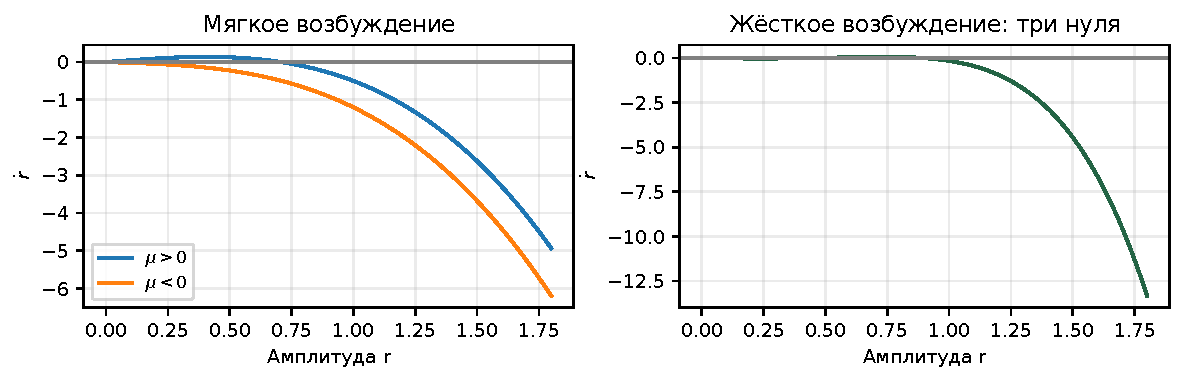
\includegraphics[width=.82\linewidth]{figures/selfosc_energy.pdf}\end{center}
